\documentclass[template.tex]{subfiles}
\usepackage{comment} 

\begin{document}

 %% \ SECTION 2
\section{The phydra package: structure \& features} \label{Section:phydrapackage}
% 2nd Section:
% Background, theoretical framework. Specifics here!
\begin{comment}
Andrew's comments: (THIS IS METHODS)
- describe modelling framework and details how you built everything
- now explain in detail what the package is \& can do, what the structure is like
- clarify that it is situated in complexity between custom scripts and modelling tools with graphical interfaces. It would be possible to design a graphical interface for this later on, but that is not the target audience.


"Python is a high-level programming language well suited to rapid development and prototyping, as well as being more accessible to domain scientists than low-level languages such as FORTRAN or C++." - Mobius GMD paper
- This is also due to the dynamic interpretation of python, which makes python slower, but python is rapidly developing and leveraging other lower level language for speed. Also has high functionality for parallelisation of code execution which is very relevant to complex marine ecosystem models. 

- clearly state limitations (scope) of phydra 
- mention that xarray-simlab is general enough to support IBMs! But not developed here.
\end{comment}


\subsection{Xarray-simlab: object-oriented modelling framework}
- Further detail on the xarray-simlab framework used for phydra!

"xarray-simlab is a Python library that provides both a generic framework for building computational models in a modular fashion and a xarray extension for setting and running simulations using the xarray.Dataset structure. It is designed for fast, interactive and exploratory modelling."

"xarray-simlab is a tool for fast model development and easy, interactive model exploration. It aims at empowering scientists to do better research in less time, collaborate efficiently and make new discoveries."

The xarray-simlab framework is built on a very few concepts that allow great flexibility in model customisation:

- models
- processes
- variables

\subsubsection{Processes}
in xarray-simlab, (almost) everything is a process.
- in the following sections, introduce the specific implementation of xarray-simlab processes within phydra, what is actually implemented in v1 and how it can be modified and used.

\subsection{phydra package}
- phydra: easy to use, open source, easy to modify, toolbox
- uses xarray-simlab processes for ALL components (for now, check again)

\subsubsection{Forcing & Physical Environment} \label{Section:PhysicalEnvironment}
- Forcing can affect one Flow, but can also affect many others, if they are related to the physical environment. This might require a additional fluxes groups defined in the components. 
- explain this here, and present what is included in phydra v1, and how the boilerplate (base classes) can be modified to create your own.
-This describes generalised mixing fluxes for nutrients and other components and provides an interface for model forcing. 
- These are aggregated via xs.group, and individual parameterisations are also possible by an EnvPar object passed in model initiation.

\subsubsection{Components}
- Components are state variables, make sure to use clear wording and explain well

\subsubsection{Flows}
- Flows are parts of differential equations, that affect one or more components, and can be influenced by forcing and the physical environment


\subsection{Model development workflow}

%%% TWO-COLUMN FIGURES
%
%%f
\begin{figure*}[t]
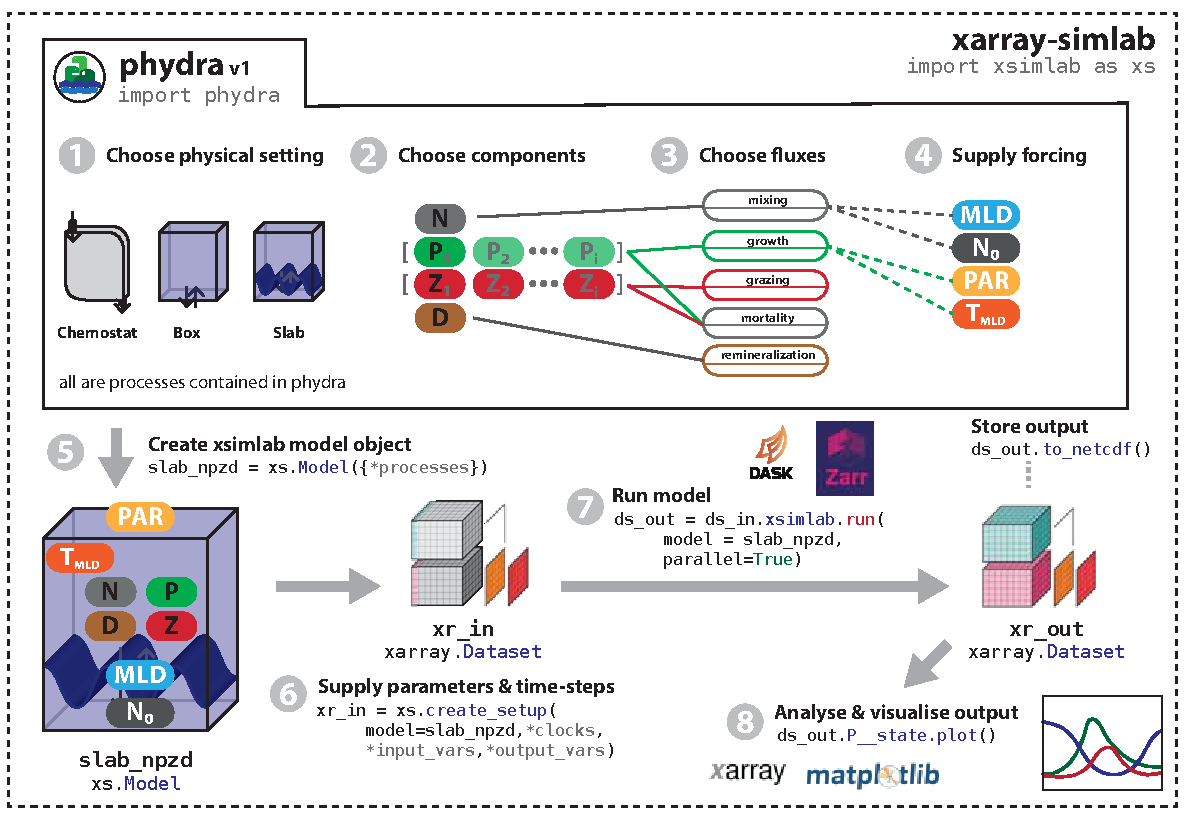
\includegraphics[width=12cm]{Figures/firstdraft_schematics/01__schematics_phydra_1.pdf}
\caption{The phydra package is embedded within the xarray-simlab framework. phydra contains a library of physical settings (1), components (i.e. state variables) (2), fluxes (3) and forcing variables (4), that can be combined and reused to create an xarray-simlab model instance. Xarray-simlab provides the functionality to define the model (5) from processes in the phydra library, supply parameters and create an xarray input (6), then run the model (7) and the resulting output is dynamically stored in another xarray, with fully labeled dimensions and containing all parameters.}
\label{phydraschematics}
\end{figure*}

general explanation, and then go into detail below (see Figure \ref{phydraschematics})

% Everything below here is optional, it depends on what I can actually do in the package
\subsubsection{Dimensionality}
- Dimensionality is a very important fact of building models, and xarray-simlab provides a simple, but sometimes tricky interface for managing dimensionality, so make sure to explain it relatively well here, as well as the implementations.
- I can cite https://www.biogeosciences.net/17/609/2020/ to explain why dimensionality is an important consideration in phytoplankton models.

\subsubsection{Runtime}
- explain what the options are to run the model, depends on if a time implicit method will be added to solve, or if it will just remain with the time explicit steps of xarray-simlab

\subsubsection{Model Diagnostics}
- this is a relevant section, *if* Benoît can help me with creating the ODE visualisation & model diagnostics.

\subsubsection{Parameter fitting}
- this is a relevant section, if i manage to get some decent parameter fitting results for the example 1 and 3.. either only 3 or both, is my feeling. 



\subsection{Forcing and verification data} \label{Section:ForcingSection}

To simplify models of complex systems larger processes are not mechanistically implemented, but instead empirically represented as an external forcing. In two of the presented use cases, we adapt a slab representation of ocean physics as defined by \citet{Evans1985ACycles}. The multi-dimensional ocean is reduced to two layers, where the upper layer provides a zero dimensional setting for our ecosystem model. The bottom layer is often assumed to contain a fixed concentration of nutrients (usually nitrate), but this can also vary with depth or time. There is constant exchange between the layers. Nutrients are usually mixing up into the upper layer, where they are consumed by phytoplankton. 

The fraction of all ecosystem components sinking to the bottom layer are lost from the system. These exchanges of water masses within this two-layered model ocean are driven by the empirically derived mixed layer depth (MLD). Additional common forcings that are used in slab models modify phytoplankton growth, e.g. metabolic rates via temperature and light harvesting via irradiance. Such forcing can situate a slab model a theoretically in any location in the global ocean. Compared to the natural habitat of marine plankton, the slab model is a radical simplification. With the appropriate forcing the resulting simulations can yield meaningful results that can be compared with bulk properties of the marine ecosystem \cite[e.g.][]{Evans1985ACycles, Fasham1990a}. 

\subsubsection{Global nutrient, light and temperature climatologies as slab model forcing}
In line with the concept of phydra as a tool for rapid prototyping of marine ecosystem models, we compiled a set of global climatological forcings for slab models. These forcings are derived from World Ocean Atlas (WOA) 2018 data and a recent global MLD climatology kindly provided by Clément de Boyer Montégut, and Moderate Resolution Imaging Spectroradiometer (MODIS-aqua) satellite data for the time period 2002–2019.

WOA data provides objectively analysed climatological mean depth profiles of nutrients (nitrate, phosphate \& silicate) and temperature on 1 \unit{°} longitude/latitude grid \cite{Garcia2019WORLDSilicate}. The values have been interpolated from data collected in the World Ocean Database and provide an empirical estimate of the biogeochemical conditions in areas of the global ocean throughout the year. WOA 2018 data is maintained and provided by NOAA (\url{https://www.nodc.noaa.gov/OC5/woa18/woa18data.html, accessed October 2019}).\\

The MLD climatology is an updated version of the original climatology presented in  \citet{deBoyerMontegut2004MixedClimatology}, collecting data up until 2014 and with a modified criterion for MLD. The analysis of profile data combines a fixed threshold criterion for temperature (0.2 \unit{°C}) and a variable threshold criterion in density (equivalent to a 0.2 \unit{°C} decrease). MLD is diagnosed as the minimum calculated depth of both criterion for each station. This ensures that both temperature and salinity are homogeneous within the mixed layer, and compensated or barrier layers do not skew the values of MLD. This combined MLD criterion corresponds to a proxy of overturning extent depth over a few days, which lends this MLD value very well as the forcing that drives the upwelling of deeper nutrients into the upper mixed layer in slab physics (Clément de Boyer Montégut, personal communication). Spatial resolution of the climatology is on a 2 \unit{°} longitude/latitude grid.\\

In addition to the oceanographic and biogeochemical parameters, the provided set of global forcings includes a global climatology of irradiance from satellite data. The NASA satellite MODIS-aqua provides the most up-to-date global climatologies of photosynthetically active radiation (PAR) \cite{MODIS-Aqua2018NASAGroup}. 
\\
With this set of forcings we can experimentally run a slab model built in phydra in (almost) any location of the ocean. MLD can be used as an empirical forcing for mixing in our slab models. Average nutrient concentration below the mixed layer, extracted from the WOA 2018 climatologies, can be used to provide a more realistic estimate of nutrient supply at certain locations throughout the year. The deep nutrient climatology averages WOA 2018 data 5 \unit{m} below closest available climatological MLD value. The final 1 \unit{°} gridded data product can be accessed via Github [provide link] and is easily integrated with models built using the phydra package. 
The monthly climatologies are spatially averaged over a selected location (see Figure \ref{phydraforcing} a) and interpolated to obtain daily values (see Figure \ref{phydraforcing} b).



% this is a custom function to be able to see references when rendering subfiles:
\biblio

\end{document}